\chapter{Ergebnis und Produktpräsentation}

Dieses Kapitel stellt das entwickelte Endprodukt vor und dokumentiert die zentralen Funktionen der Anwendung in ihrer fertigen Form. Im Unterschied zu einer klassischen empirischen Evaluation steht hier weniger die statistische Messung im Mittelpunkt, sondern die fachlich belastbare und visuell nachvollziehbare Produktwirkung. Ziel ist es, das entstandene Werkzeug als nutzbares Ergebnis eines engineering-orientierten Entwicklungsprozesses zu präsentieren und damit die praktische Umsetzung der fachlichen Anforderungen sichtbar zu machen.

\section{Entwickeltes Endprodukt}

Die entwickelte Webanwendung stellt einen interaktiven Scheduling-Visualizer dar, der verschiedene präemptive CPU-Scheduling-Verfahren in einem gemeinsamen Lern- und Analysekontext verknüpft. Die Anwendung erlaubt es, Prozessen mit Ankunftszeit, Burst-Zeit, Priorität und weiteren Attributen ein Szenario zu definieren, einen Algorithmus auszuwählen und den Ablauf zeitlich sichtbar zu machen.

Das fertige Produkt verbindet damit drei zentrale Aspekte:

\begin{itemize}
    \item technische Korrektheit der Scheduling-Logik,
    \item verständliche Darstellung des zeitlichen Ablaufs,
    \item und eine nutzerorientierte Oberfläche für Lehr- und Vergleichszwecke.
\end{itemize}

Damit erfüllt die Anwendung nicht nur die fachlichen Vorgaben eines Betriebssystem-Kapitels, sondern stellt zugleich ein tragfähiges und erweitertes Produkt dar, das im Studienkontext als didaktisches Werkzeug eingesetzt werden kann.

\section{Produktüberblick und Nutzerfluss}

Der typische Nutzerfluss beginnt mit dem Definieren eines Szenarios. Auf der Startseite sind die Systemgrundlagen, die Eingabeform und die Auswahl relevanter Prozessparameter direkt sichtbar. Nach dem Laden eines Szenarios kann der Nutzer den gewünschten Algorithmus auswählen und den Ablauf in verschiedenen Modi starten. Anschließend stehen eine Fokusansicht und eine Vergleichsübersicht zur Verfügung.

Die Anwendung wurde bewusst so aufgebaut, dass die Interaktion in logischer Reihenfolge abläuft: Eingabe, Auswahl, Ablaufsteuerung, Analyse und Vergleich. Dadurch bleibt der Nutzer bei jedem Schritt im Kontext des jeweiligen Lernziels und muss keine unnötigen Bedienhürden überwinden.

\section{Produktpräsentation mit Screenshots}

\begin{figure}[htbp]
    \centering
    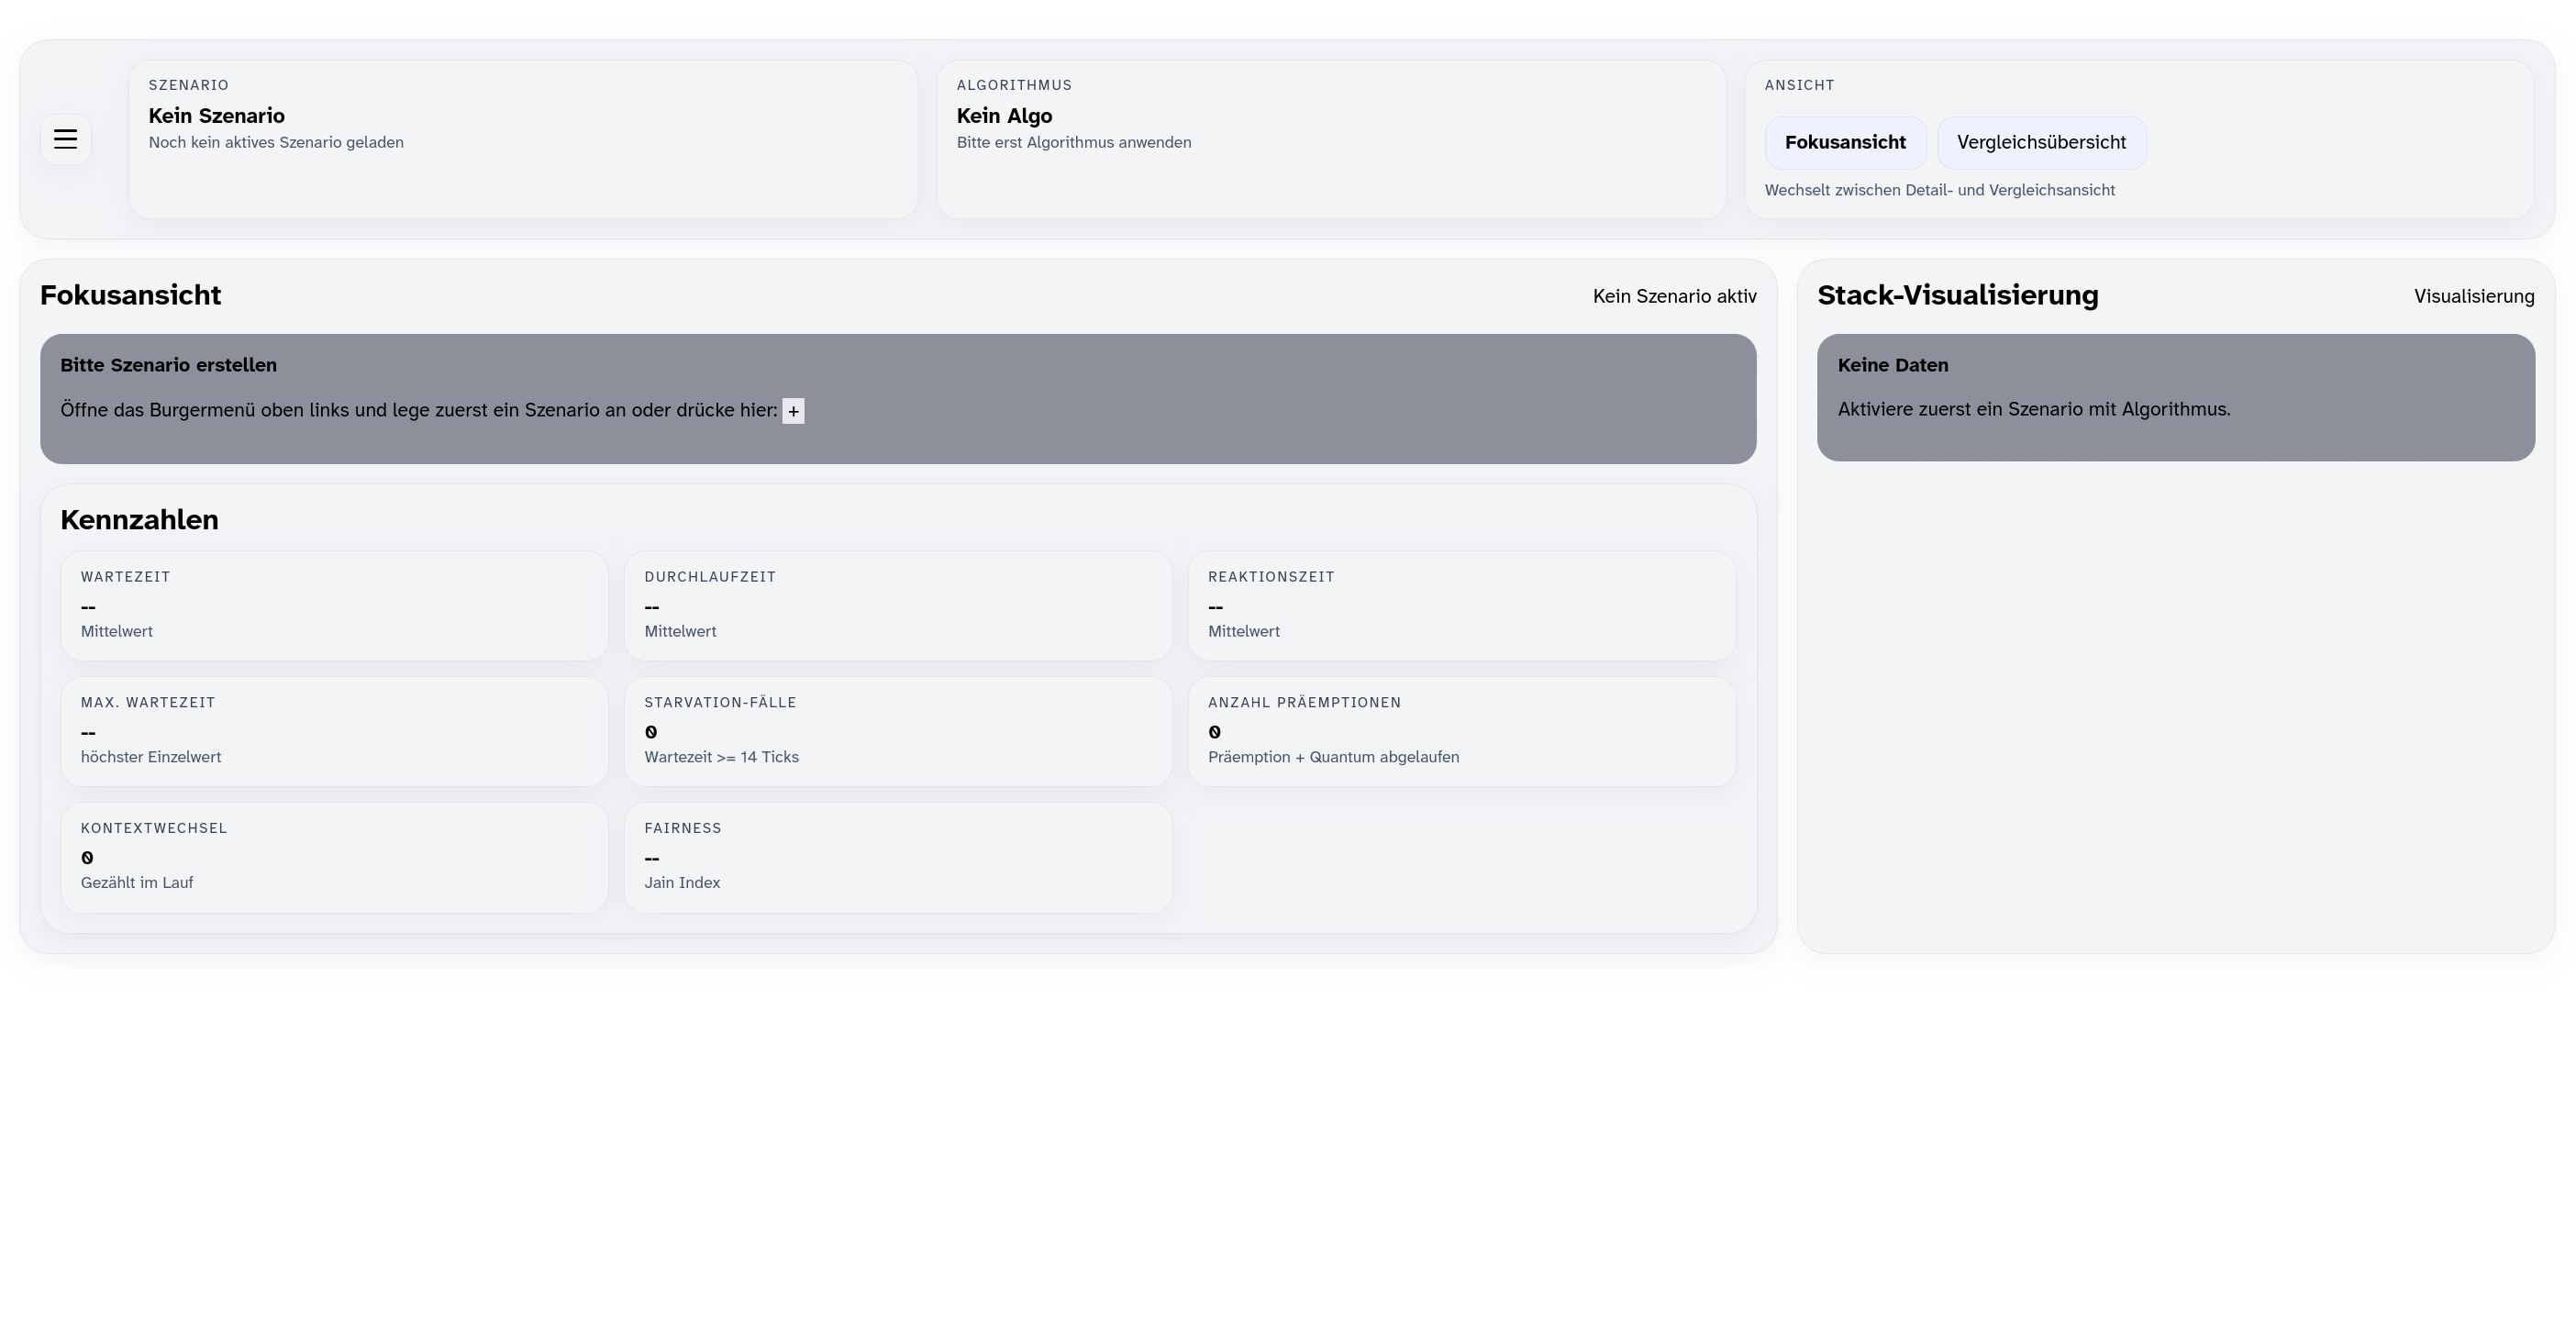
\includegraphics[width=\textwidth]{images/screenshot-ausgangslage.png}
    \caption{Startansicht der Anwendung mit leerem Zustand und erklärender Ausgangslage. Der Nutzer startet mit der Definition eines Szenarios und der Auswahl eines Scheduling-Verfahrens.}
    \label{fig:produkt-start}
\end{figure}

\begin{figure}[htbp]
    \centering
    
\includegraphics[width=\textwidth]{images/screenshot-szenario-geladen.png}
    \caption{Ladezustand eines konfigurierten Szenarios. Die Prozessdaten sind sichtbar, und die Simulation kann mit einer klaren Ablaufsteuerung initialisiert werden.}
    \label{fig:produkt-szenario}
\end{figure}

\begin{figure}[htbp]
    \centering
    
\includegraphics[width=\textwidth]{images/screenshot-fokusansicht.png}
    \caption{Fokusansicht der Simulation mit Gantt-Zeitachse, aktiver Prozessdarstellung und Kennzahlbereich. Diese Ansicht zeigt den Ablauf des gewählten Scheduling-Verfahrens in einer verständlichen, zeitlich strukturierten Form.}
    \label{fig:produkt-fokus}
\end{figure}

\begin{figure}[htbp]
    \centering
    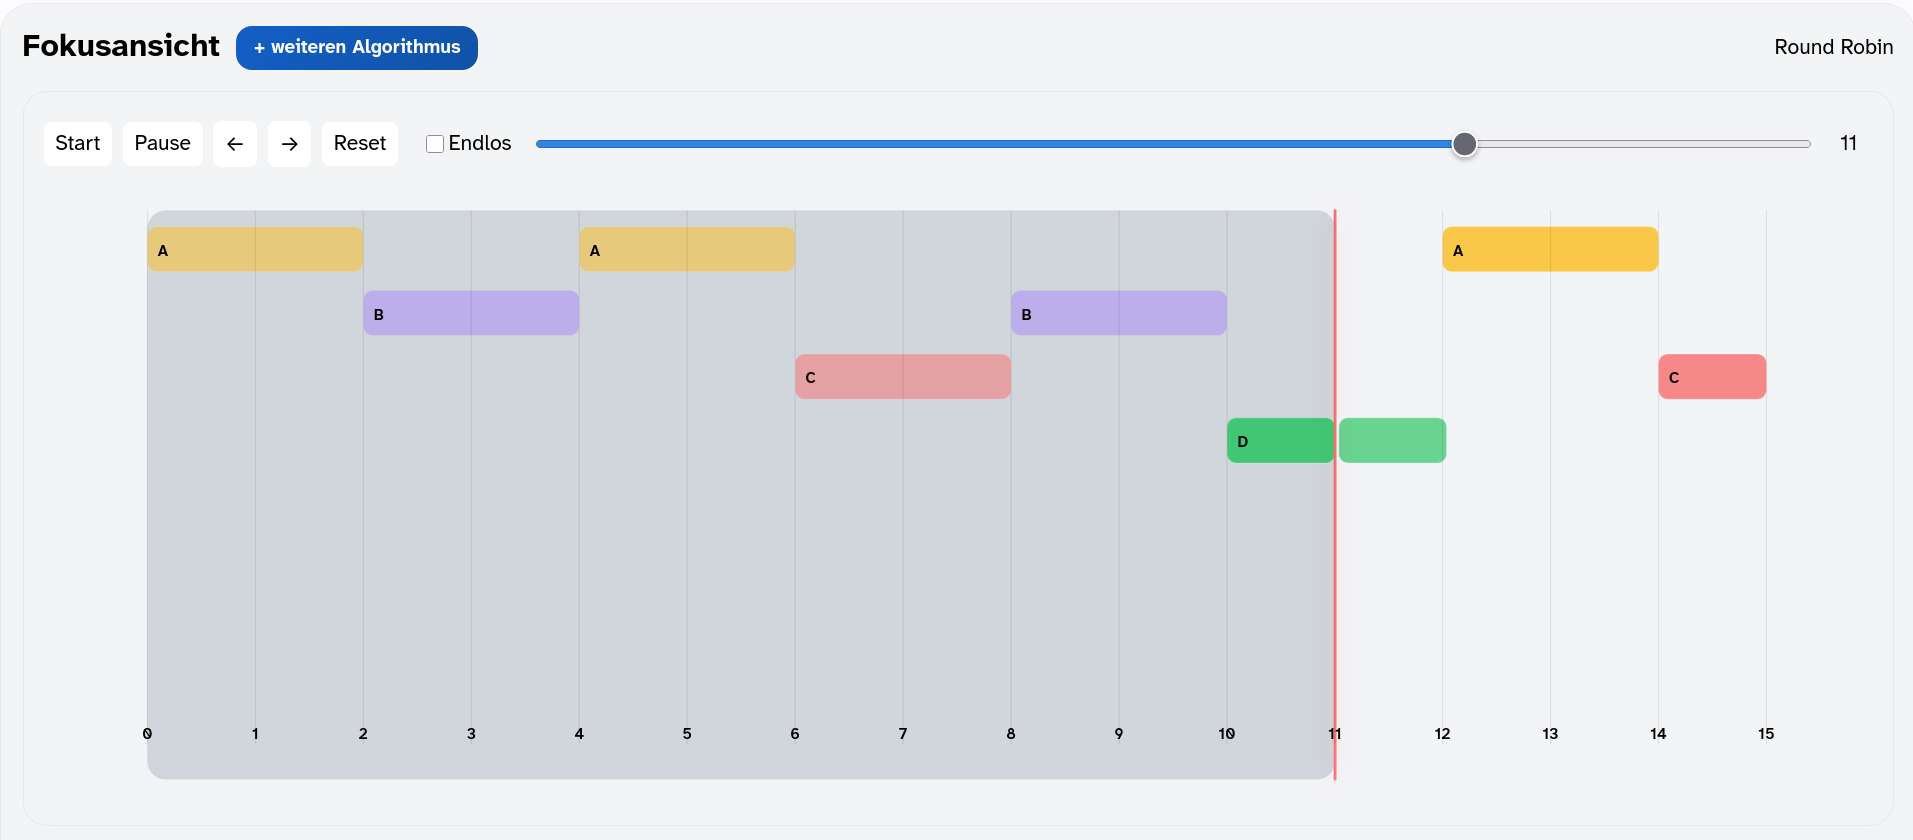
\includegraphics[width=\textwidth]{images/screenshot-gantt-detail.png}
    \caption{Detailansicht der Gantt-Darstellung. Einzelne Ausführungssegmente, Präemptionen und Prozesswechsel werden als konkrete Zeitabschnitte sichtbar gemacht.}
    \label{fig:produkt-gantt}
\end{figure}

\begin{figure}[htbp]
    \centering
    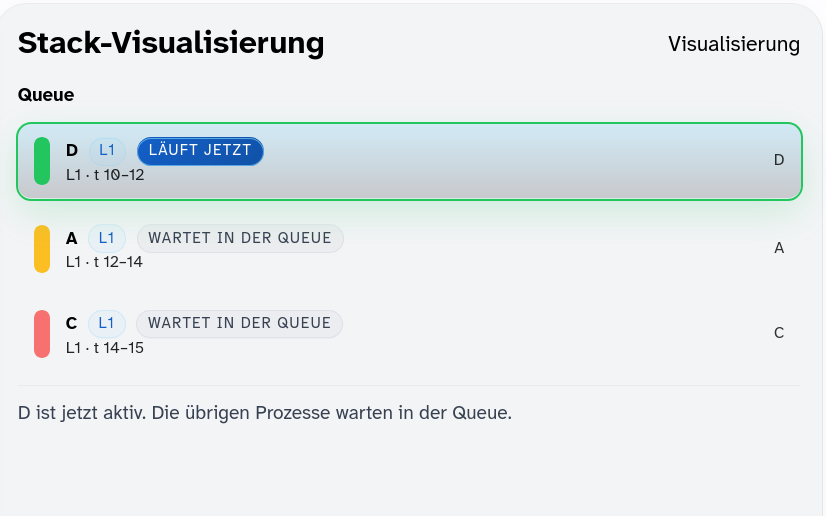
\includegraphics[width=\textwidth]{images/screenshot-stack-detail.png}
    \caption{Darstellung des Prozessstatus in der Warteschlangenansicht. Der aktuelle Zustand und die Warteliste werden gleichzeitig präsentiert, wodurch die Auswahlentscheidung des Algorithmus nachvollziehbar wird.}
    \label{fig:produkt-stack}
\end{figure}

\begin{figure}[htbp]
    \centering
    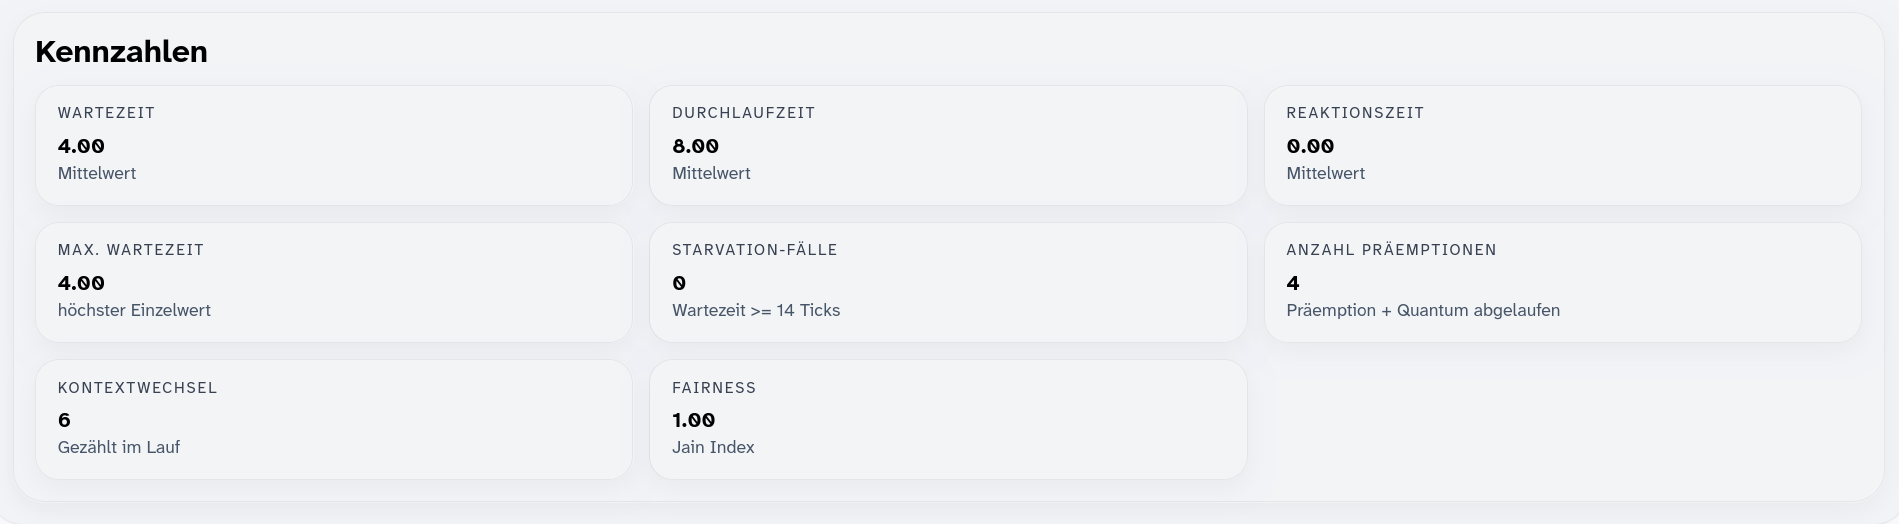
\includegraphics[width=\textwidth]{images/screenshot-kennzahlen-detail.png}
    \caption{Kennzahlenbereich mit Warte-, Durchlauf- und Reaktionszeiten. Die Metriken geben eine kompakte fachliche Bewertung des Simulationslaufs wieder.}
    \label{fig:produkt-kennzahlen}
\end{figure}

\begin{figure}[htbp]
    \centering
    
\includegraphics[width=\textwidth]{images/screenshot-vergleichsuebersicht-gesamt.png}
    \caption{Vergleichsübersicht mit mehreren Läufen unter identischem Szenario. Die Darstellung ermöglicht den praktischen Vergleich verschiedener Scheduling-Verfahren anhand des selben Dateninputs.}
    \label{fig:produkt-vergleich}
\end{figure}

\section{Umgesetzte Funktionalität}

Die fertige Anwendung erfüllt die wesentlichen Anforderungen, die im Verlauf der Arbeit aus fachlicher, didaktischer und HCI-orientierter Sicht definiert wurden. Zu den wichtigsten Funktionen gehören:

\begin{itemize}
    \item Erstellung und Bearbeitung von Prozessdaten mit Ankunftszeit, Burst-Zeit und Priorität,
    \item interaktive Szenariogenerierung mit vordefinierten Basis-Szenarien und direkter Vorschau,
    \item Auswahl und Vergleich verschiedener Scheduling-Verfahren über einen klaren Algorithmusdialog,
    \item kontrollierte Wiedergabe mit Start, Pause, Schrittmodus und Zeitsprung,
    \item visuelle Darstellung als Zeitachsenmodell in Gantt-Form,
    \item Ausgabe relevanter Kennzahlen pro Ablauf,
    \item Vergleich mehrerer Läufe auf identischem Szenario mit Bewertungs- und Matrixansicht.
\end{itemize}

Diese Funktionen zeigen, dass die Anwendung als echtes Produkt und nicht nur als akademische Demonstration umgesetzt wurde. Sie ermöglicht fachliche Analyse, didaktische Nachvollziehbarkeit und konkrete Produktnutzung in einem integrativen Ablauf, wobei die Benutzerführung durch Szenario-Generator, Vergleichsansichten und strukturierte Bedienpfade zusätzlich gestärkt wird.

\section{Ergebnisbetrachtung}

Das endständige Produkt erfüllt die ursprüngliche Zielsetzung der Arbeit: Es macht die Dynamik präemptiver Scheduling-Verfahren anschaulich, verständlich und vergleichbar. Die wichtigsten fachlichen Effekte, etwa Präemption, Kontextwechsel, Prioritätsverzug und Wartezeiten, werden nicht nur als Zahlenwerte gezeigt, sondern auch im zeitlichen Ablauf sichtbar gemacht.

Diese Kombination aus technischer Korrektheit und visueller Transparenz ist für das Produkt besonders wertvoll. Der Nutzer sieht nicht nur das Ergebnis eines Algorithmus, sondern auch die Entscheidungspfade, die zu diesem Ergebnis geführt haben. Dadurch wird die Anwendung zu einem nutzbaren Werkzeug für Lehre, Demonstration und fachliche Erörterung.

Das Produkt zeigt außerdem, dass die Arbeit eine konkrete technische Leistung erbracht hat: Es wurde eine vollständig nutzbare, interaktive Anwendung entwickelt, die fachlich korrekte Simulation, verständliche Visualisierung und eine klare, strukturiert gestaltete Benutzerführung verbindet. Gerade diese Kombination ist im Studiengang als engineering-orientierte Leistung besonders aussagekräftig, weil sie den Übergang von abstrakter Theorie zu konkreter Softwarelösung sichtbar macht.

Die Produktpräsentation zeigt zugleich, dass die Bachelorarbeit nicht nur ein theoretisches Dokument, sondern ein konkret umgesetztes Softwaresystem ist. Diese Perspektive passt zur engineering-orientierten Ausrichtung der Arbeit und entspricht zugleich dem fachlichen Anspruch des Studiengangs, in dem methodische Genauigkeit, technische Umsetzung und verständlicher Produktaufbau gleichwertig berücksichtigt werden müssen.
